

\begin{figure}
	\begin{minipage}{0.46\linewidth}
		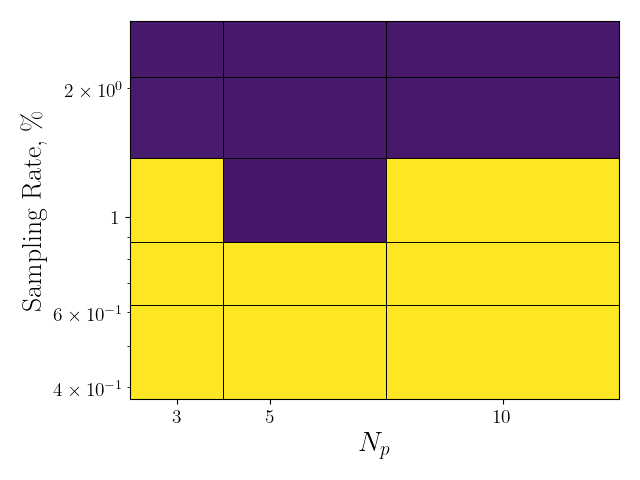
\includegraphics[width=0.99\linewidth]{Chapters/AdaptiveResults/Images/cvrc/errContours/err_contour_iter2.png}
		\subcaption{$\updateFreq = 2$}
	\end{minipage}
	\begin{minipage}{0.53\linewidth}
		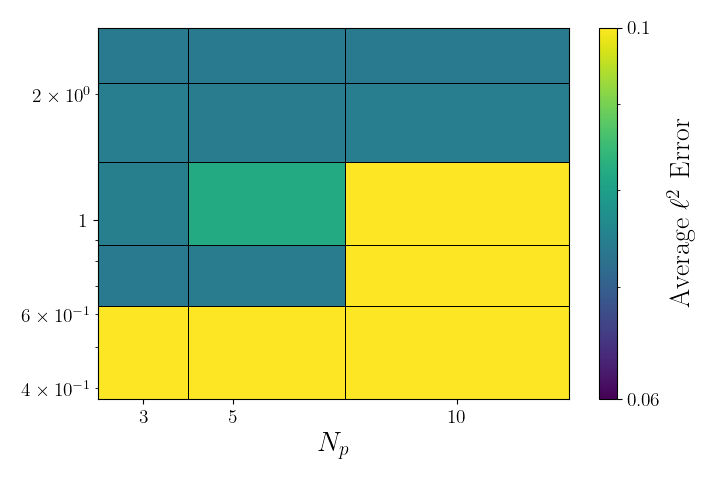
\includegraphics[width=0.99\linewidth]{Chapters/AdaptiveResults/Images/cvrc/errContours/err_contour_iter3.png}
		\subcaption{$\updateFreq = 3$}
	\end{minipage}

	\begin{minipage}{0.46\linewidth}
		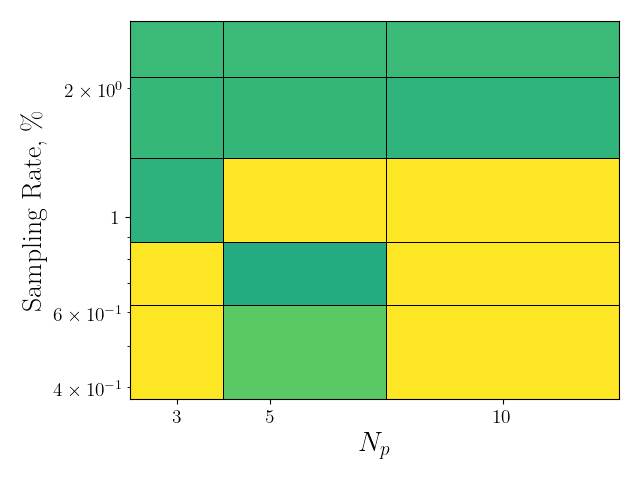
\includegraphics[width=0.99\linewidth]{Chapters/AdaptiveResults/Images/cvrc/errContours/err_contour_iter4.png}
		\subcaption{$\updateFreq = 4$}
	\end{minipage}
	\begin{minipage}{0.53\linewidth}
		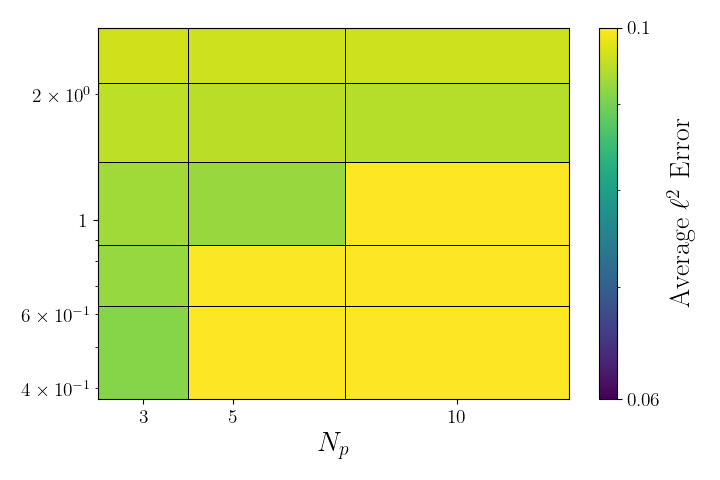
\includegraphics[width=0.99\linewidth]{Chapters/AdaptiveResults/Images/cvrc/errContours/err_contour_iter5.png}
		\subcaption{$\updateFreq = 5$}
	\end{minipage}
	\caption{\label{fig:cvrcAdaptiveROMErrContour}CVRC adaptive HPROM time-average error contours with respect to trial basis dimension and sampling rate, various $\updateFreq$.}
\end{figure}

\begin{figure}
    \begin{minipage}{0.49\linewidth}
        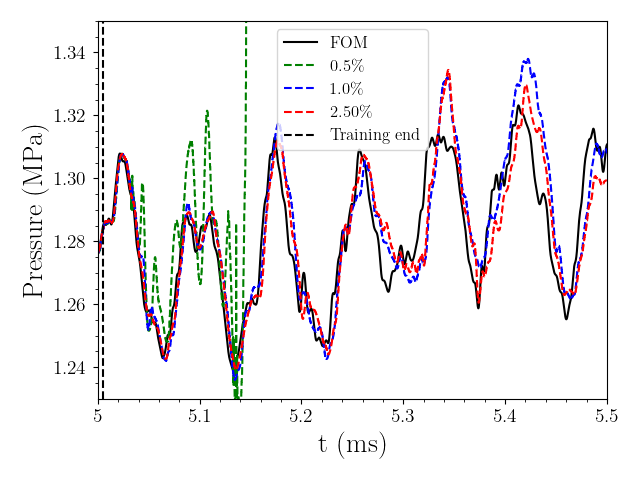
\includegraphics[width=0.99\linewidth]{Chapters/AdaptiveResults/Images/cvrc/pressure_probe_wrt_sampling.png}
        \subcaption{$\updateFreq = 3$, various $\numSamps$.}
    \end{minipage}
    \begin{minipage}{0.49\linewidth}
        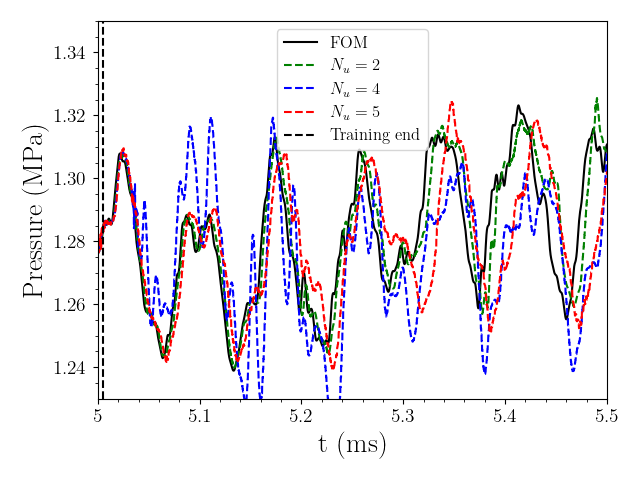
\includegraphics[width=0.99\linewidth]{Chapters/AdaptiveResults/Images/cvrc/pressure_probe_wrt_iter.png}
        \subcaption{$\numSamps = 1.0\%$, various $\updateFreq$.}
    \end{minipage}
    \caption{CVRC adaptive HPROM pressure probes, $\numPrimModes = 5$.}
\end{figure}

\begin{figure}
	\begin{minipage}{0.99\linewidth}
		\raisebox{-0.5\height}{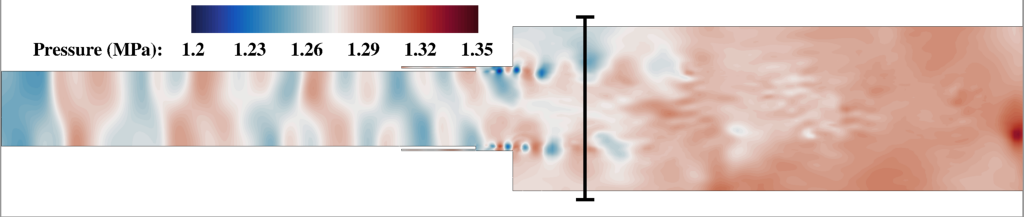
\includegraphics[width=0.84\linewidth,trim={0.5em 0.5em 0.5em 0.5em},clip]{Chapters/AdaptiveResults/Images/cvrc/fieldContours/fom_pressure_z.png}}
		\raisebox{-0.5\height}{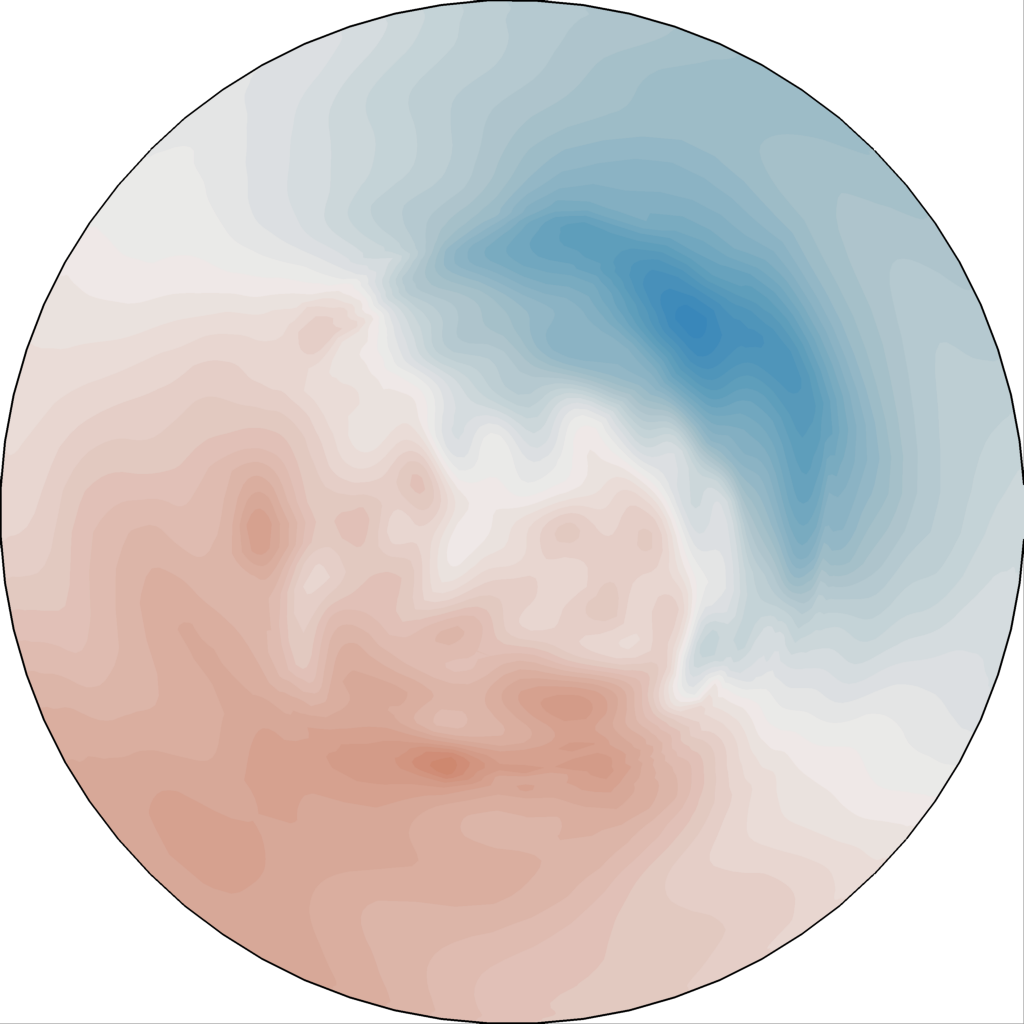
\includegraphics[width=0.14\linewidth,trim={0.0em 0.1em 0.0em 0.1em},clip]{Chapters/AdaptiveResults/Images/cvrc/fieldContours/fom_pressure_x.png}}
	\end{minipage}
    \begin{minipage}{0.99\linewidth}
		\raisebox{-0.5\height}{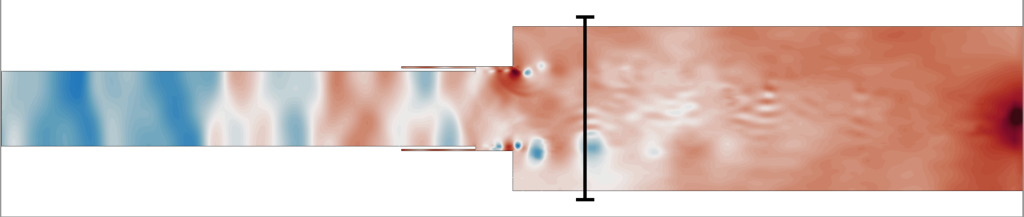
\includegraphics[width=0.84\linewidth,trim={0.5em 0.5em 0.5em 0.5em},clip]{Chapters/AdaptiveResults/Images/cvrc/fieldContours/adapt_iter2_pressure_z.png}}
		\raisebox{-0.5\height}{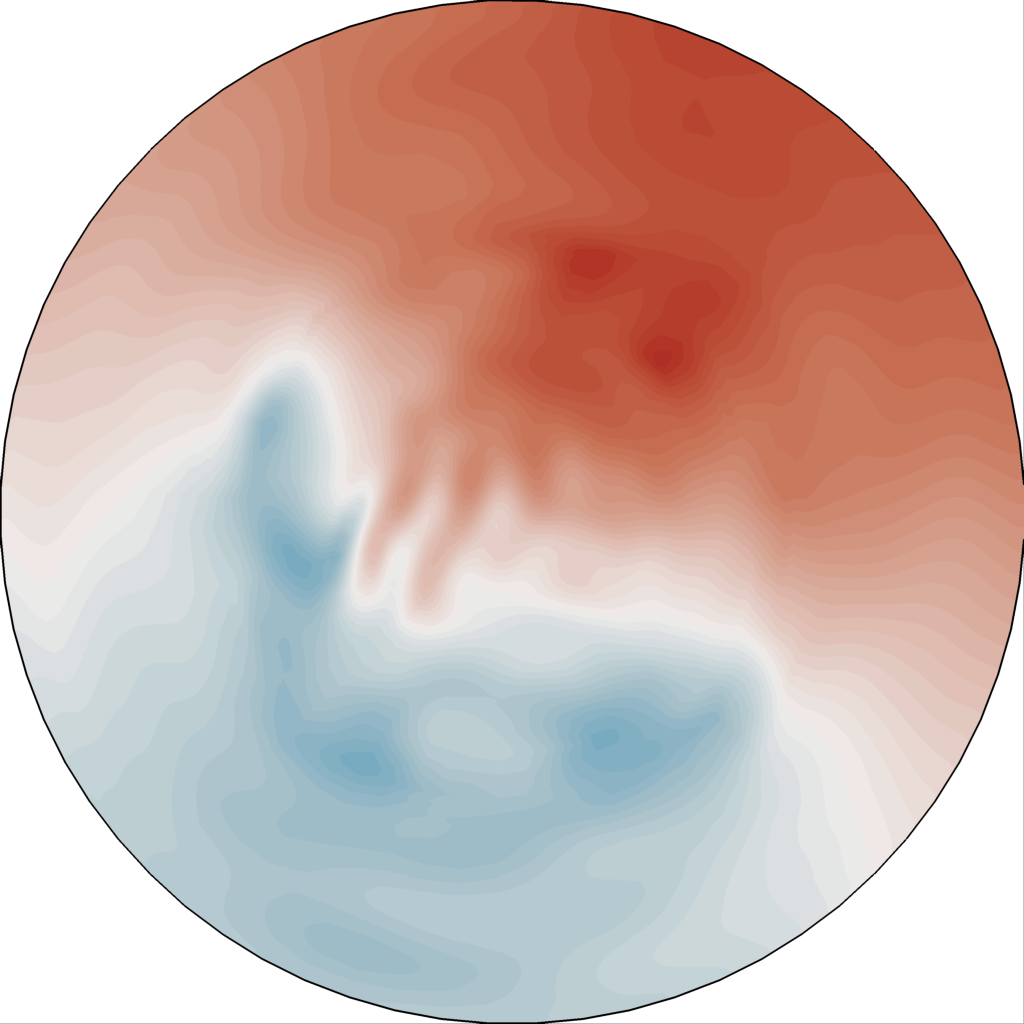
\includegraphics[width=0.14\linewidth,trim={0.0em 0.1em 0.0em 0.1em},clip]{Chapters/AdaptiveResults/Images/cvrc/fieldContours/adapt_iter2_pressure_x.png}}
	\end{minipage}
    \begin{minipage}{0.99\linewidth}
		\raisebox{-0.5\height}{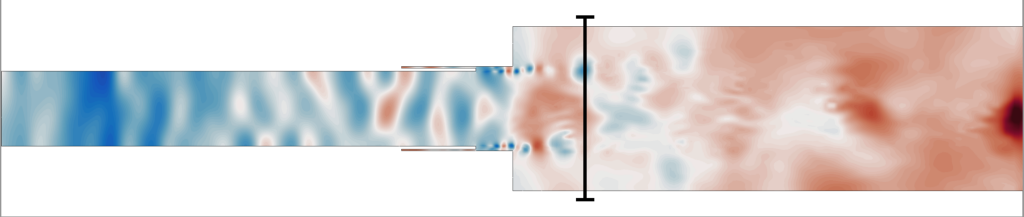
\includegraphics[width=0.84\linewidth,trim={0.5em 0.5em 0.5em 0.5em},clip]{Chapters/AdaptiveResults/Images/cvrc/fieldContours/adapt_iter4_pressure_z.png}}
		\raisebox{-0.5\height}{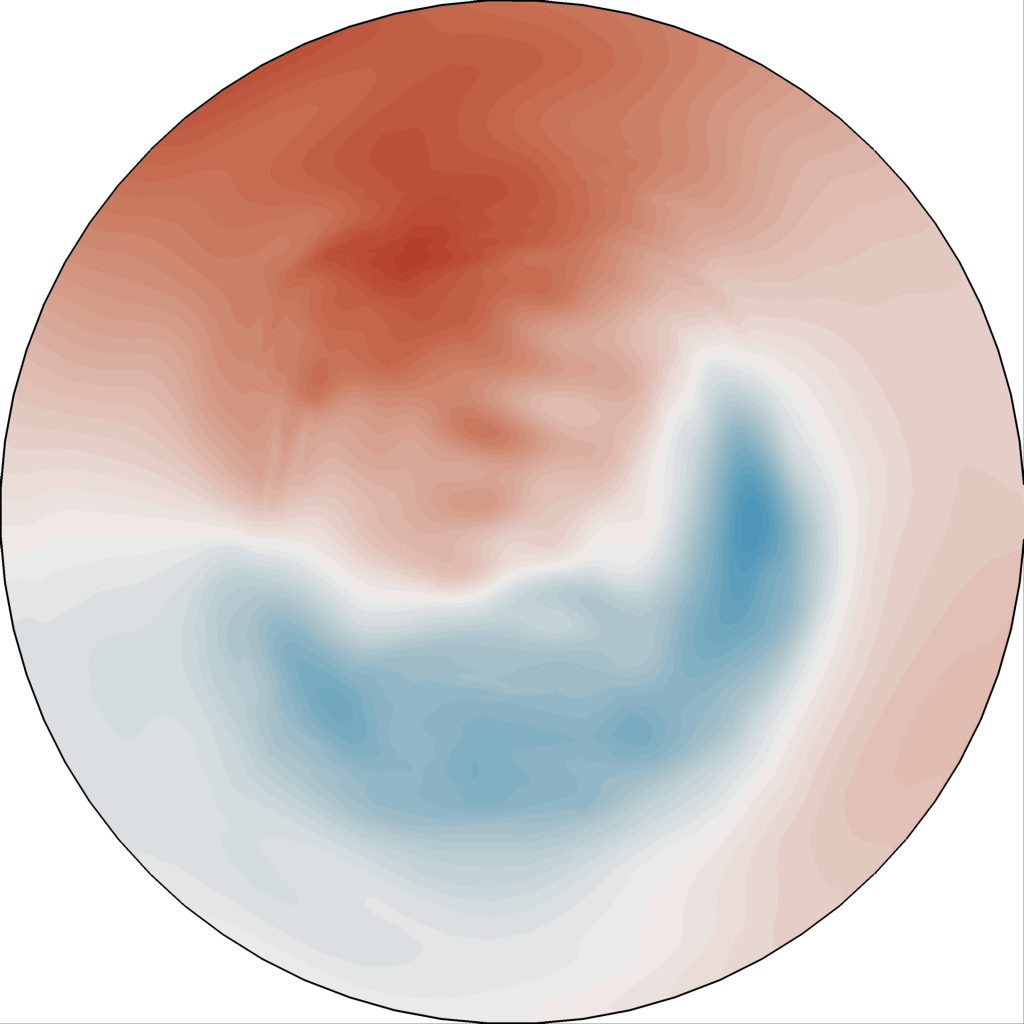
\includegraphics[width=0.14\linewidth,trim={0.0em 0.1em 0.0em 0.1em},clip]{Chapters/AdaptiveResults/Images/cvrc/fieldContours/adapt_iter4_pressure_x.png}}
	\end{minipage}
    \begin{minipage}{0.99\linewidth}
		\raisebox{-0.5\height}{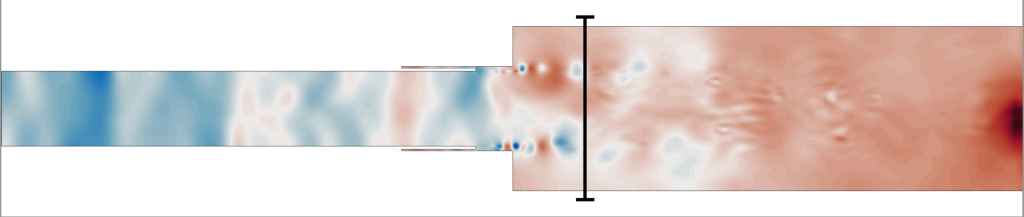
\includegraphics[width=0.84\linewidth,trim={0.5em 0.5em 0.5em 0.5em},clip]{Chapters/AdaptiveResults/Images/cvrc/fieldContours/adapt_iter5_pressure_z.png}}
		\raisebox{-0.5\height}{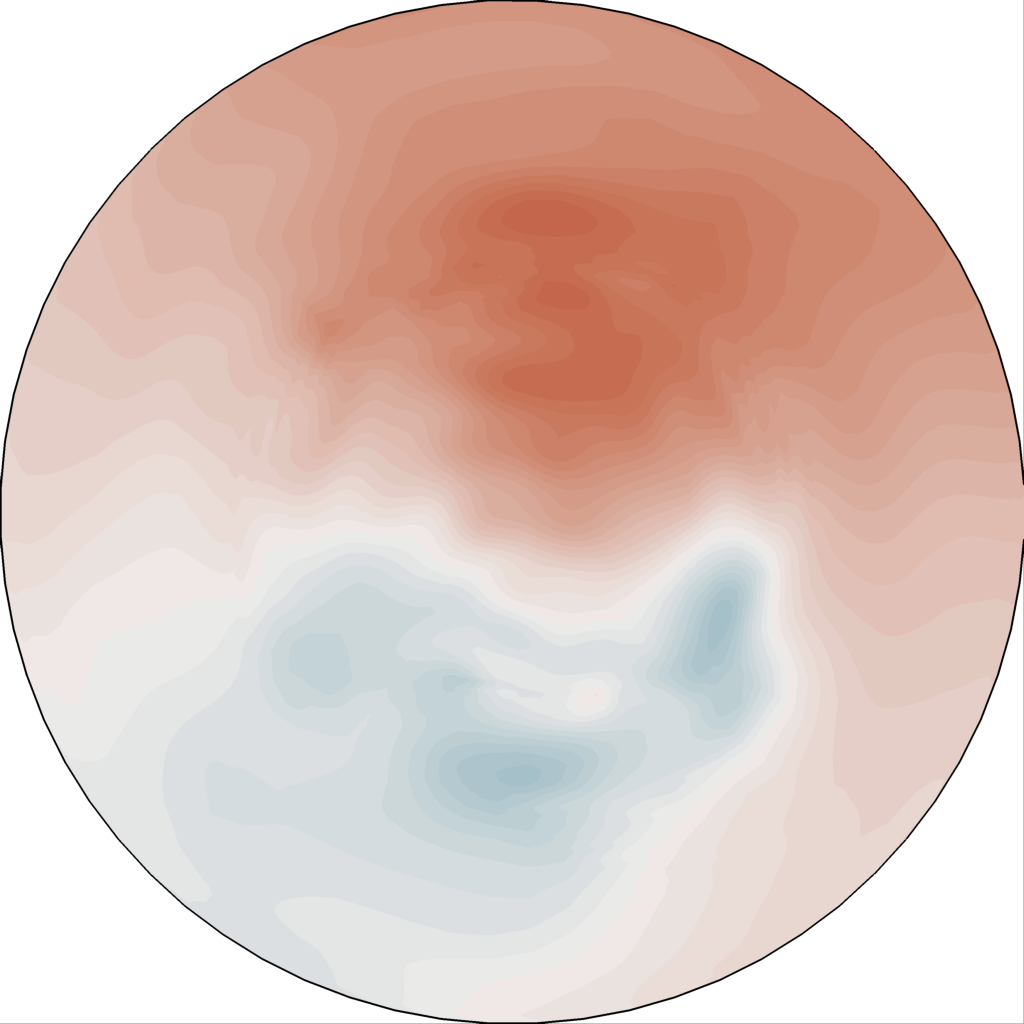
\includegraphics[width=0.14\linewidth,trim={0.0em 0.1em 0.0em 0.1em},clip]{Chapters/AdaptiveResults/Images/cvrc/fieldContours/adapt_iter5_pressure_x.png}}
	\end{minipage}
    \caption{CVRC pressure field $\timeVar = 5.5$ ms, XXX, XXX. From top to bottom: FOM, XXX, XXX, XXX.}
\end{figure}

\begin{figure}
	\begin{minipage}{0.99\linewidth}
		\raisebox{-0.5\height}{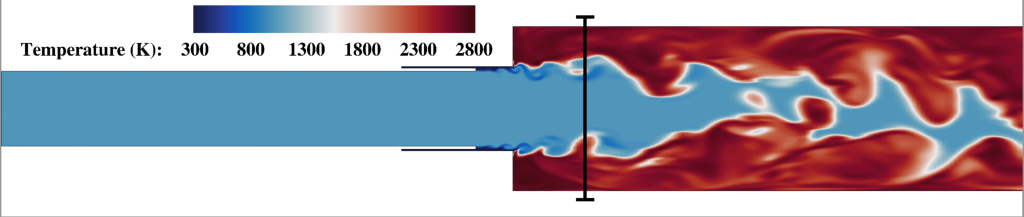
\includegraphics[width=0.84\linewidth,trim={0.5em 0.5em 0.5em 0.5em},clip]{Chapters/AdaptiveResults/Images/cvrc/fieldContours/fom_temperature_z.png}}
		\raisebox{-0.5\height}{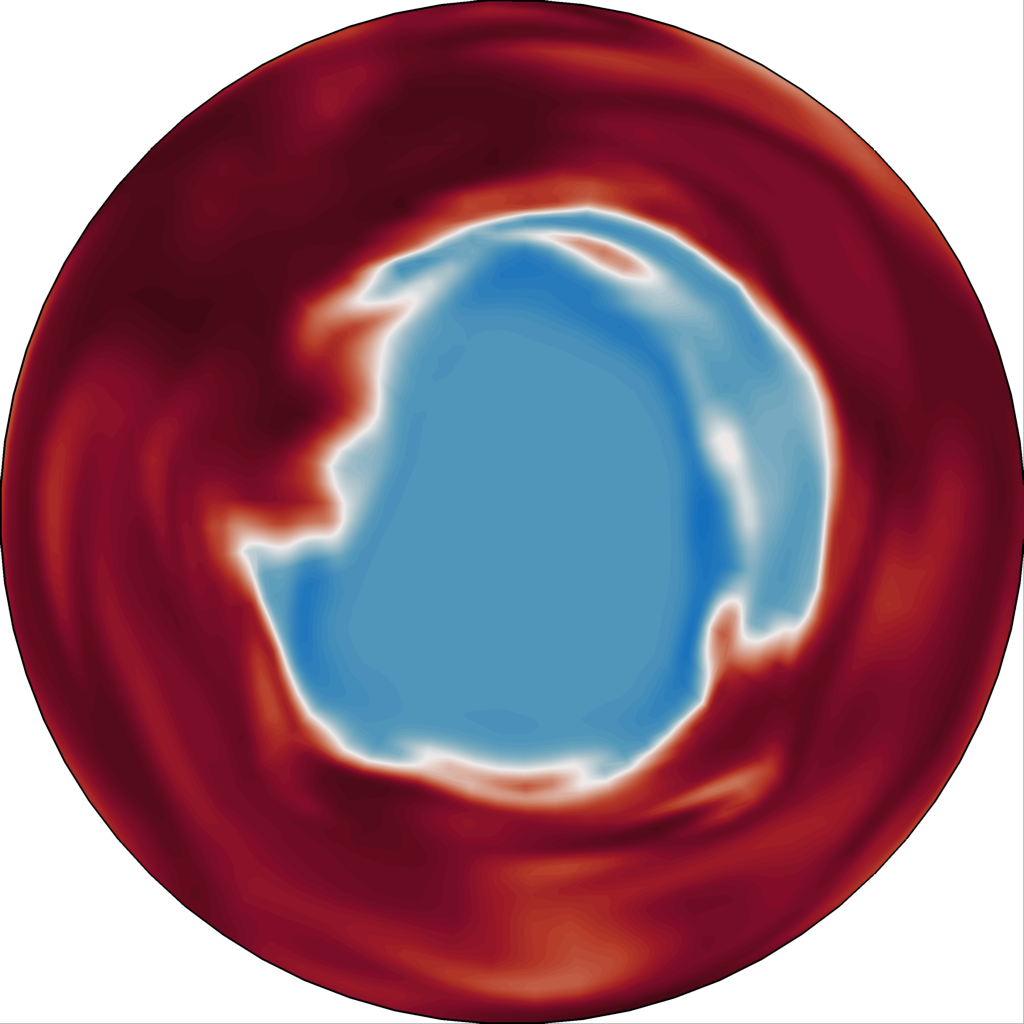
\includegraphics[width=0.14\linewidth,trim={0.0em 0.1em 0.0em 0.1em},clip]{Chapters/AdaptiveResults/Images/cvrc/fieldContours/fom_temperature_x.png}}
	\end{minipage}
    \begin{minipage}{0.99\linewidth}
		\raisebox{-0.5\height}{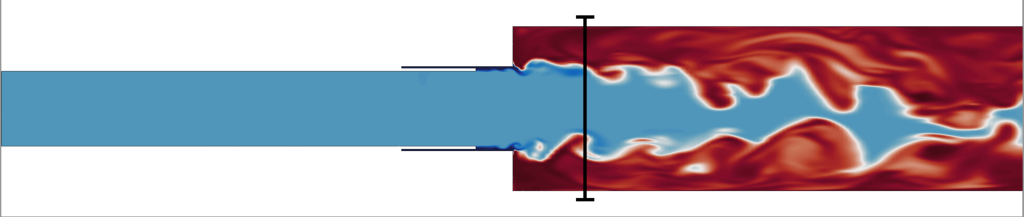
\includegraphics[width=0.84\linewidth,trim={0.5em 0.5em 0.5em 0.5em},clip]{Chapters/AdaptiveResults/Images/cvrc/fieldContours/adapt_iter2_temperature_z.png}}
		\raisebox{-0.5\height}{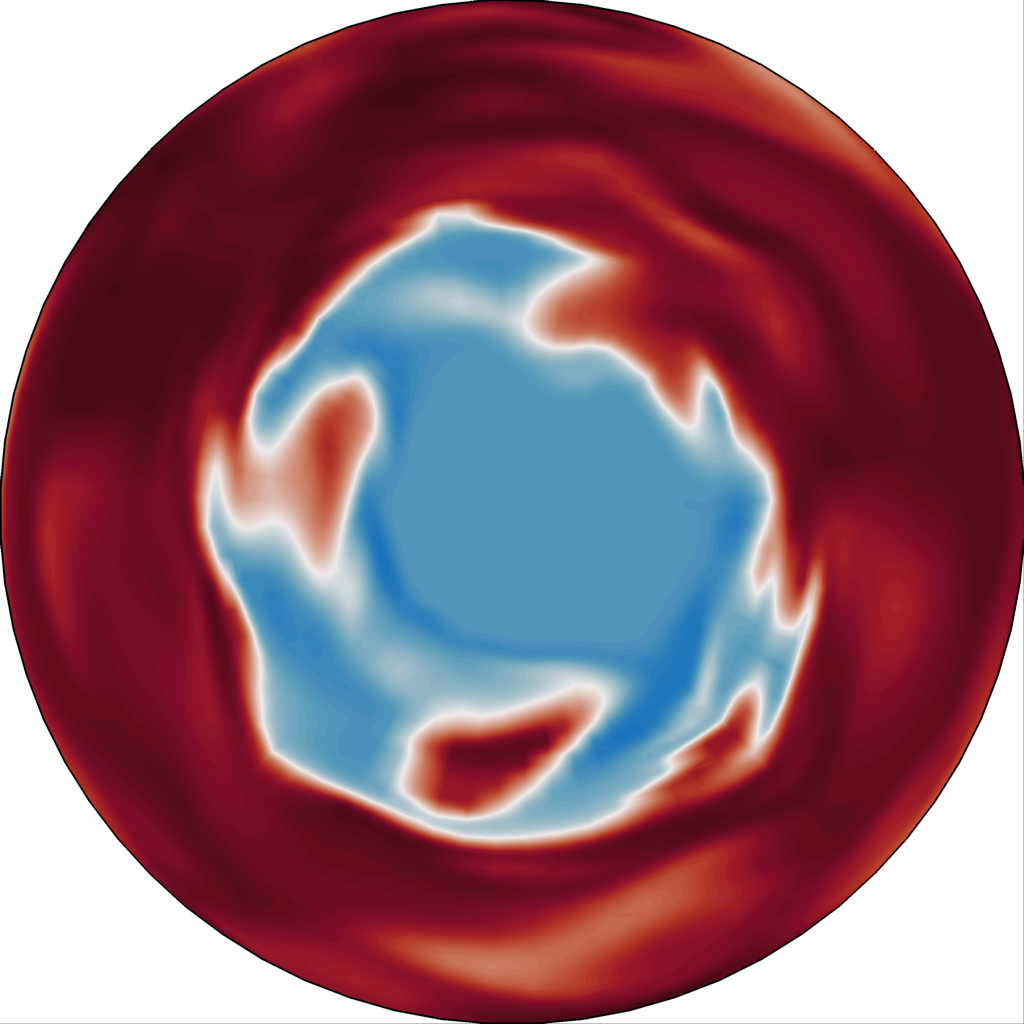
\includegraphics[width=0.14\linewidth,trim={0.0em 0.1em 0.0em 0.1em},clip]{Chapters/AdaptiveResults/Images/cvrc/fieldContours/adapt_iter2_temperature_x.png}}
	\end{minipage}
    \begin{minipage}{0.99\linewidth}
		\raisebox{-0.5\height}{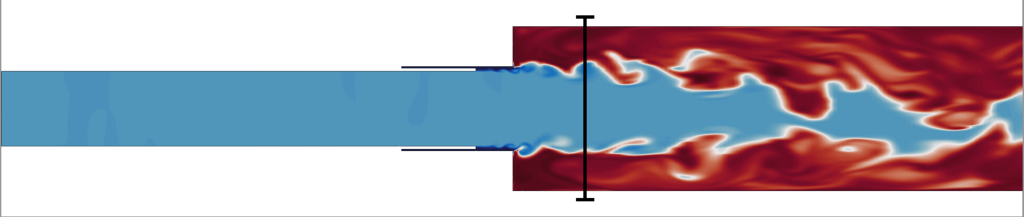
\includegraphics[width=0.84\linewidth,trim={0.5em 0.5em 0.5em 0.5em},clip]{Chapters/AdaptiveResults/Images/cvrc/fieldContours/adapt_iter4_temperature_z.png}}
		\raisebox{-0.5\height}{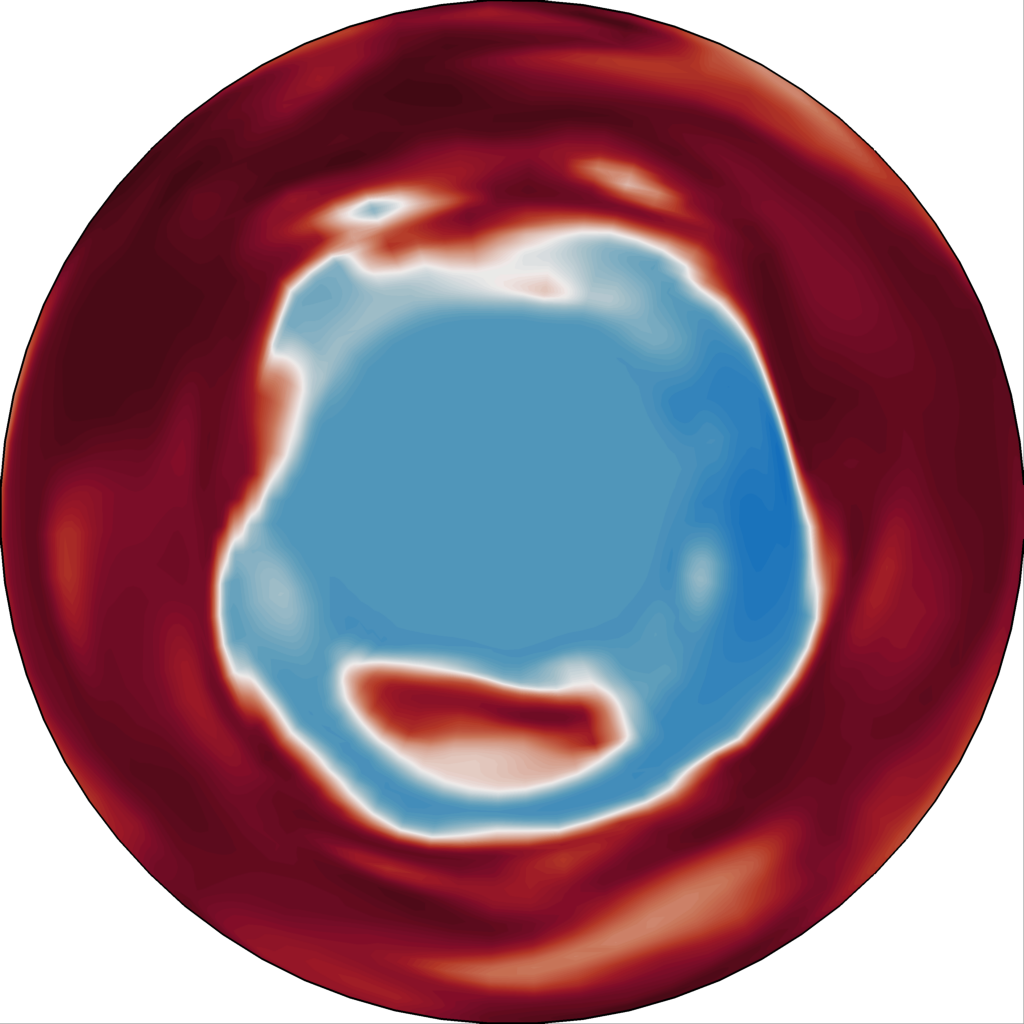
\includegraphics[width=0.14\linewidth,trim={0.0em 0.1em 0.0em 0.1em},clip]{Chapters/AdaptiveResults/Images/cvrc/fieldContours/adapt_iter4_temperature_x.png}}
	\end{minipage}
    \begin{minipage}{0.99\linewidth}
		\raisebox{-0.5\height}{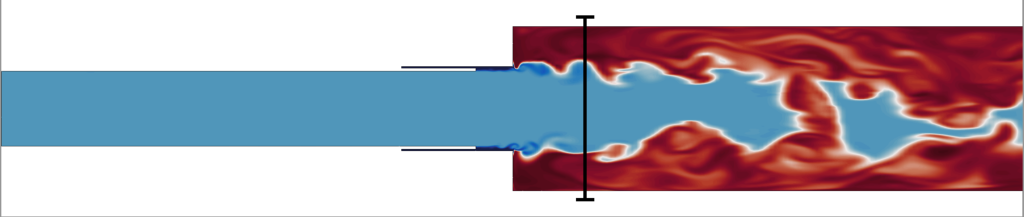
\includegraphics[width=0.84\linewidth,trim={0.5em 0.5em 0.5em 0.5em},clip]{Chapters/AdaptiveResults/Images/cvrc/fieldContours/adapt_iter5_temperature_z.png}}
		\raisebox{-0.5\height}{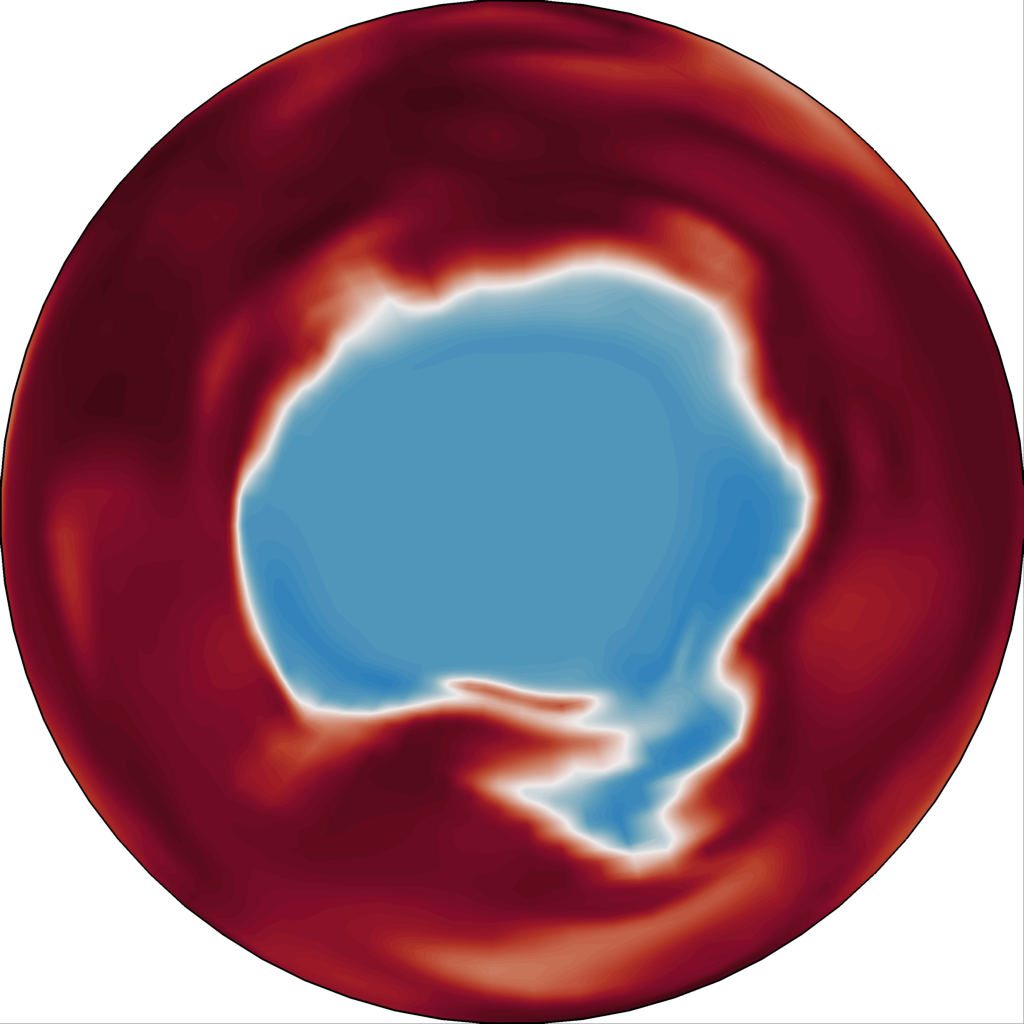
\includegraphics[width=0.14\linewidth,trim={0.0em 0.1em 0.0em 0.1em},clip]{Chapters/AdaptiveResults/Images/cvrc/fieldContours/adapt_iter5_temperature_x.png}}
	\end{minipage}
    \caption{CVRC temperature field $\timeVar = 5.5$ ms, XXX, XXX. From top to bottom: FOM, XXX, XXX, XXX.}
\end{figure}

\begin{figure}
	\begin{minipage}{0.99\linewidth}
		\raisebox{-0.5\height}{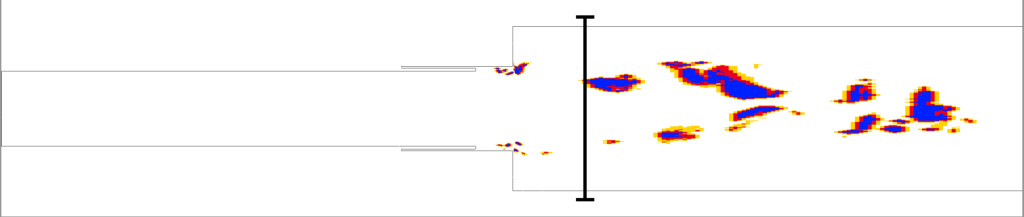
\includegraphics[width=0.84\linewidth,trim={0.5em 0.5em 0.5em 0.5em},clip]{Chapters/AdaptiveResults/Images/cvrc/iblank/iblank_z_1025.png}}
		\raisebox{-0.5\height}{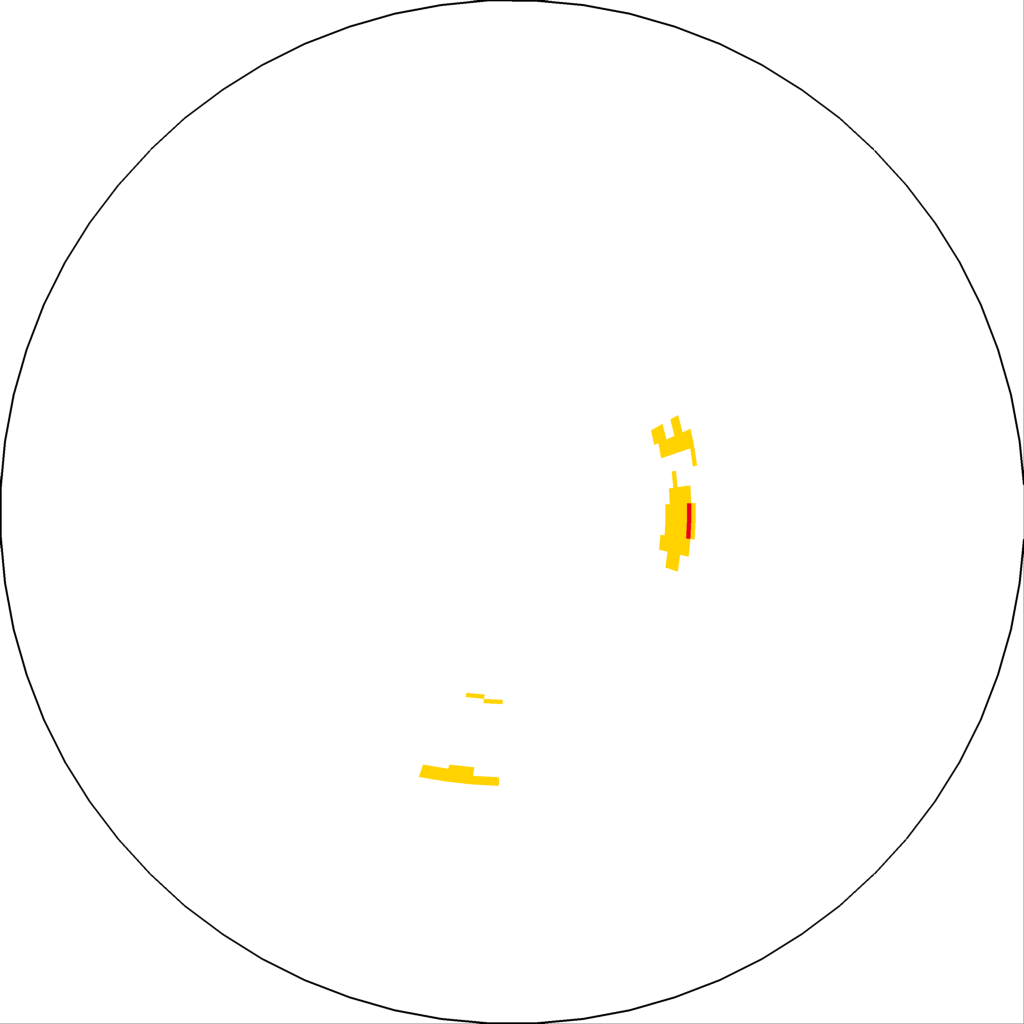
\includegraphics[width=0.14\linewidth,trim={0.0em 0.1em 0.0em 0.1em},clip]{Chapters/AdaptiveResults/Images/cvrc/iblank/iblank_x_1025.png}}
	\end{minipage}
    \begin{minipage}{0.99\linewidth}
		\raisebox{-0.5\height}{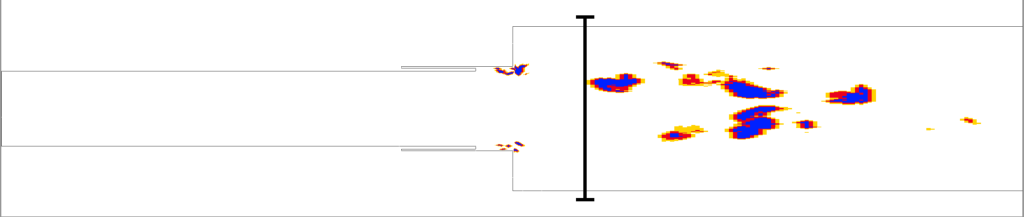
\includegraphics[width=0.84\linewidth,trim={0.5em 0.5em 0.5em 0.5em},clip]{Chapters/AdaptiveResults/Images/cvrc/iblank/iblank_z_1050.png}}
		\raisebox{-0.5\height}{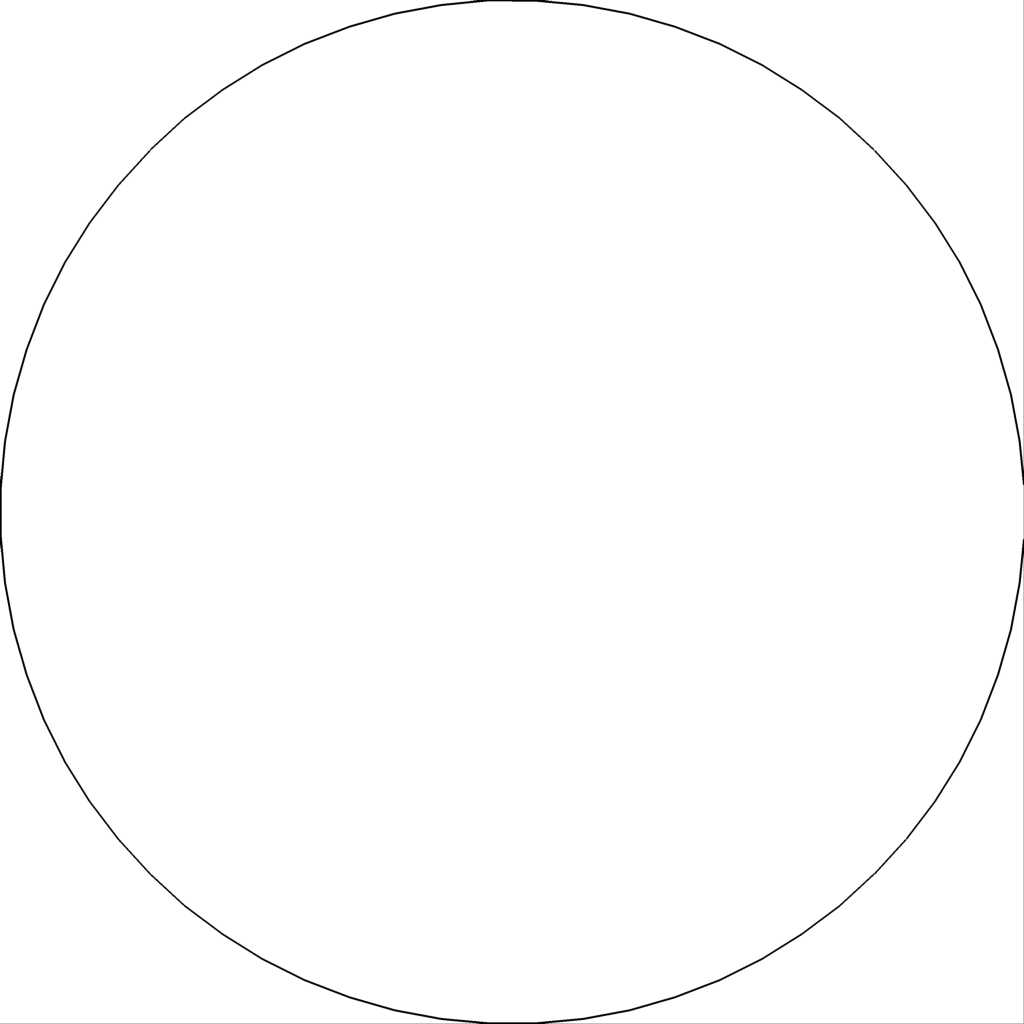
\includegraphics[width=0.14\linewidth,trim={0.0em 0.1em 0.0em 0.1em},clip]{Chapters/AdaptiveResults/Images/cvrc/iblank/iblank_x_1050.png}}
	\end{minipage}
    \begin{minipage}{0.99\linewidth}
		\raisebox{-0.5\height}{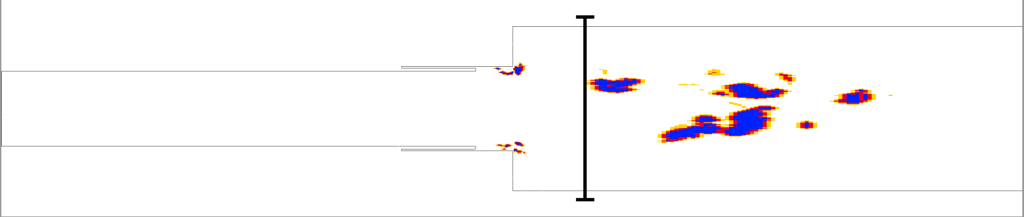
\includegraphics[width=0.84\linewidth,trim={0.5em 0.5em 0.5em 0.5em},clip]{Chapters/AdaptiveResults/Images/cvrc/iblank/iblank_z_1075.png}}
		\raisebox{-0.5\height}{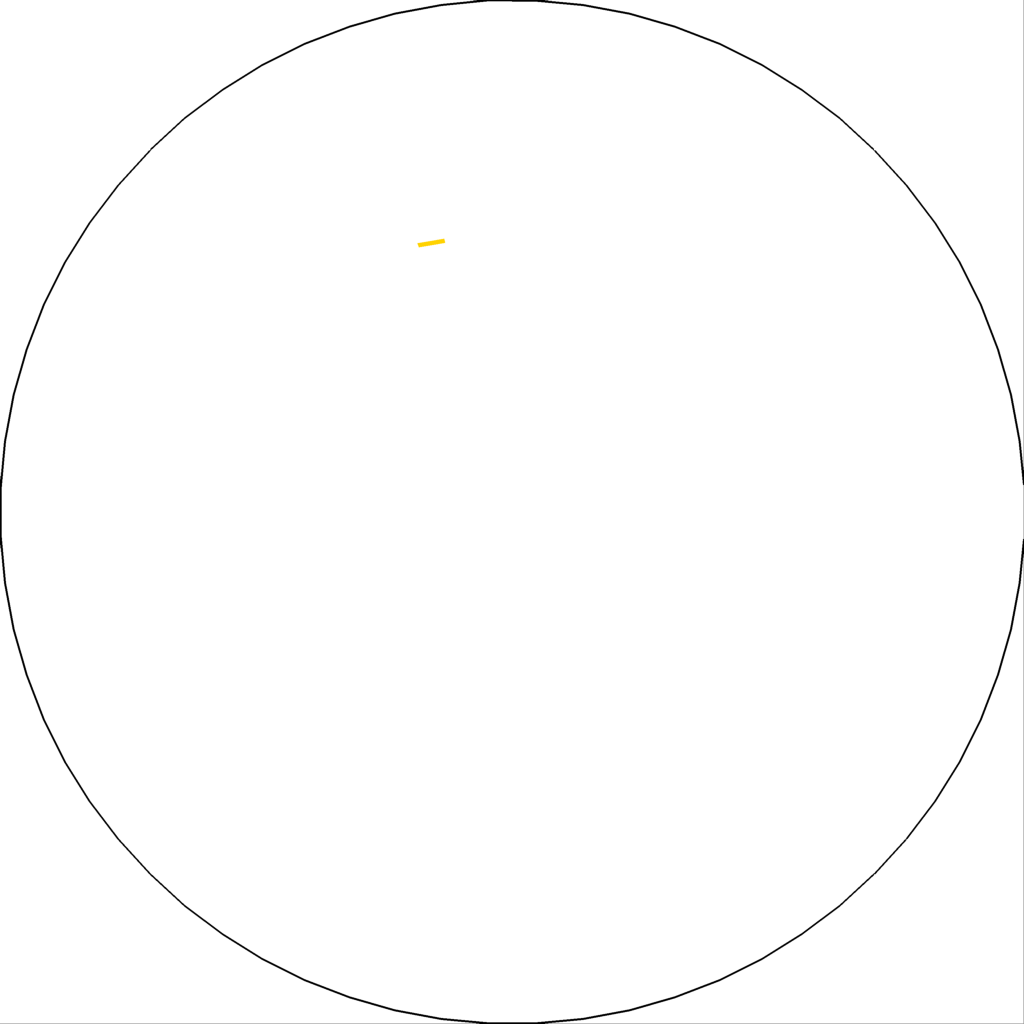
\includegraphics[width=0.14\linewidth,trim={0.0em 0.1em 0.0em 0.1em},clip]{Chapters/AdaptiveResults/Images/cvrc/iblank/iblank_x_1075.png}}
	\end{minipage}
    \begin{minipage}{0.99\linewidth}
		\raisebox{-0.5\height}{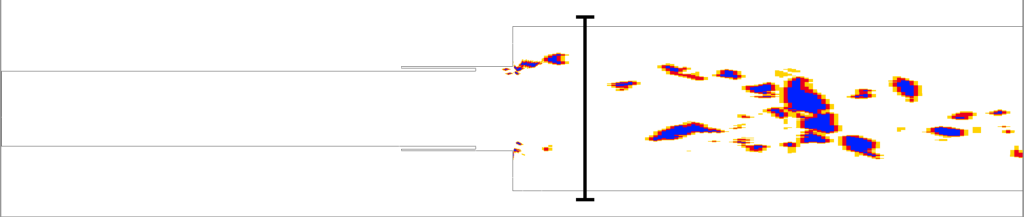
\includegraphics[width=0.84\linewidth,trim={0.5em 0.5em 0.5em 0.5em},clip]{Chapters/AdaptiveResults/Images/cvrc/iblank/iblank_z_1100.png}}
		\raisebox{-0.5\height}{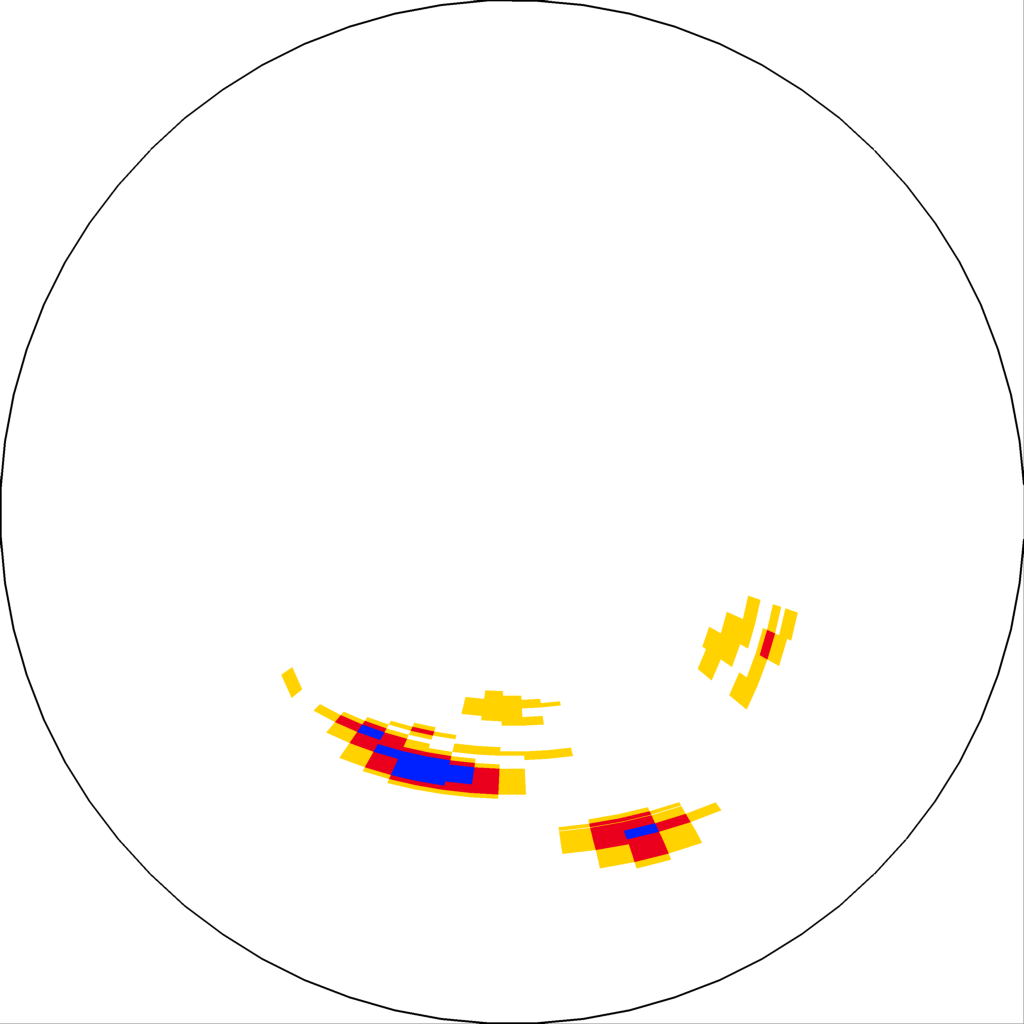
\includegraphics[width=0.14\linewidth,trim={0.0em 0.1em 0.0em 0.1em},clip]{Chapters/AdaptiveResults/Images/cvrc/iblank/iblank_x_1100.png}}
	\end{minipage}
    \caption{CVRC sample mesh, XXX, XXX. From top to bottom, $\timeVar = XXX$, $XXX$, $XXX$, $XXX$.}
\end{figure}

\begin{figure}
	\centering
	\begin{minipage}{0.45\linewidth}
		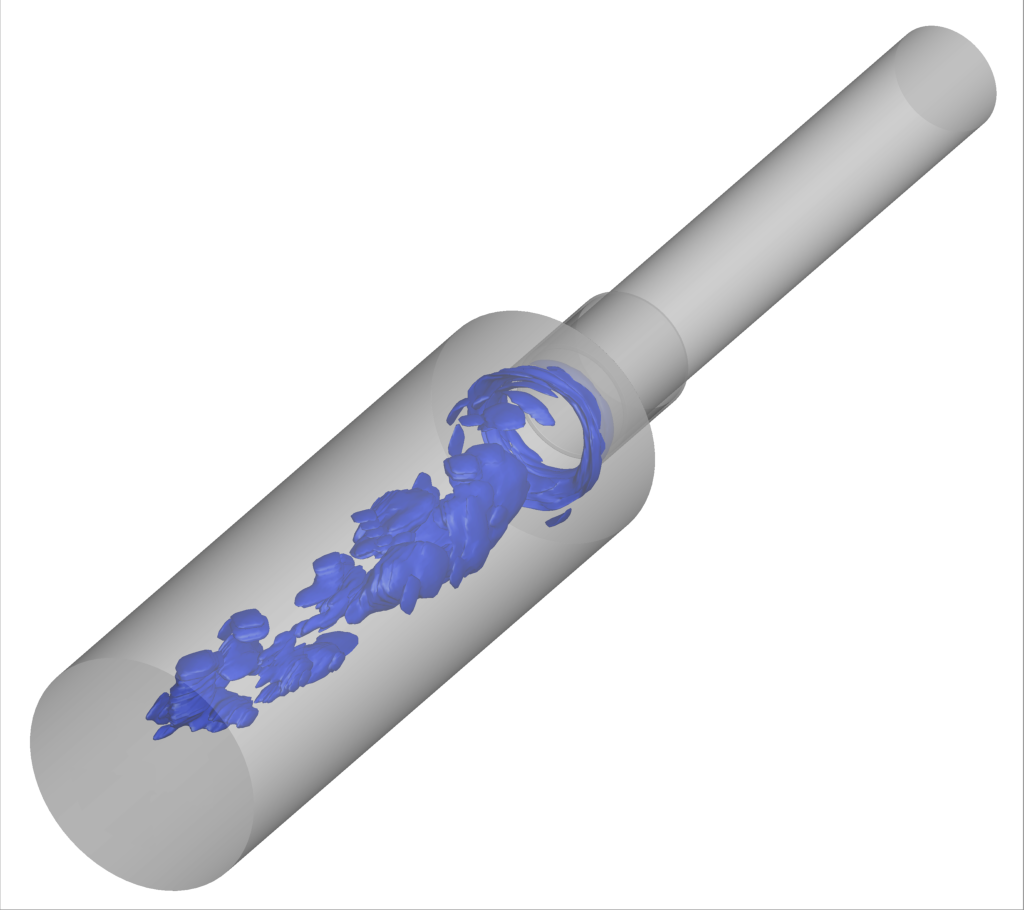
\includegraphics[width=0.99\linewidth,trim={0.5em 0.5em 0.5em 0.5em},clip]{Chapters/AdaptiveResults/Images/cvrc/iblank/iblank_iso_1025.png}
	\end{minipage}
	\begin{minipage}{0.45\linewidth}
		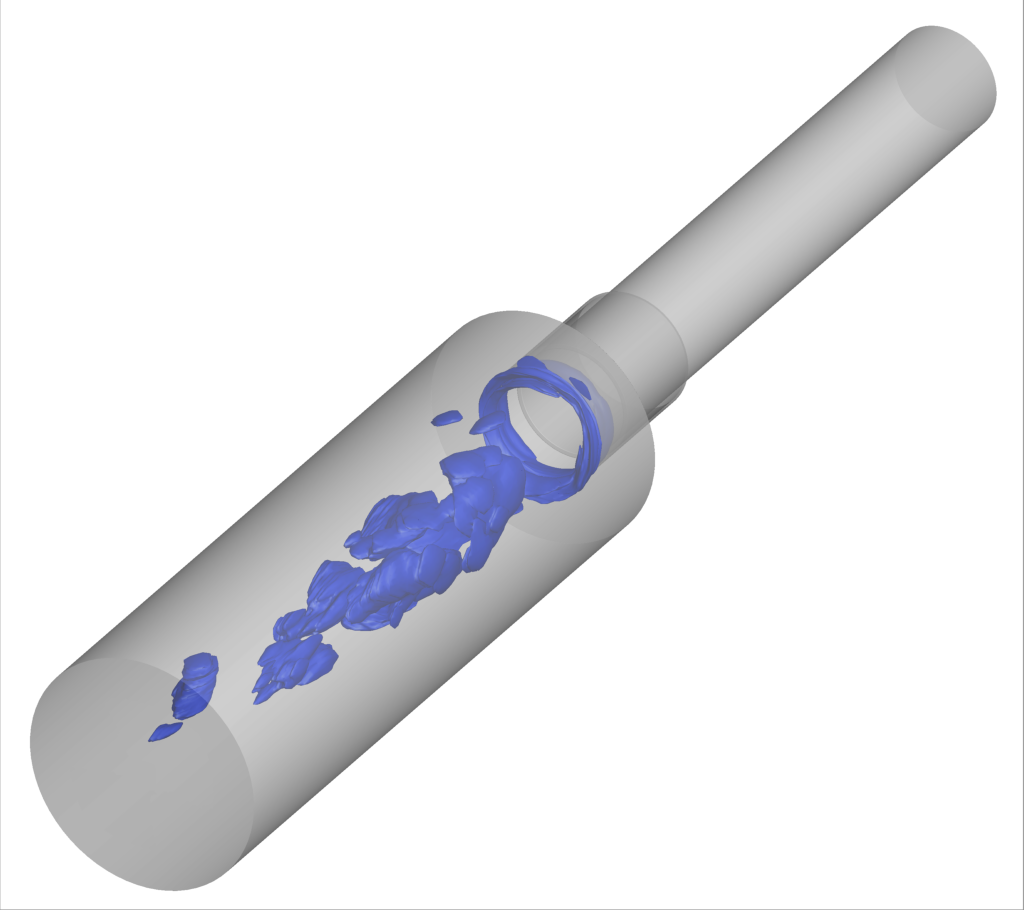
\includegraphics[width=0.99\linewidth,trim={0.5em 0.5em 0.5em 0.5em},clip]{Chapters/AdaptiveResults/Images/cvrc/iblank/iblank_iso_1050.png}
	\end{minipage}

	\centering
	\begin{minipage}{0.45\linewidth}
		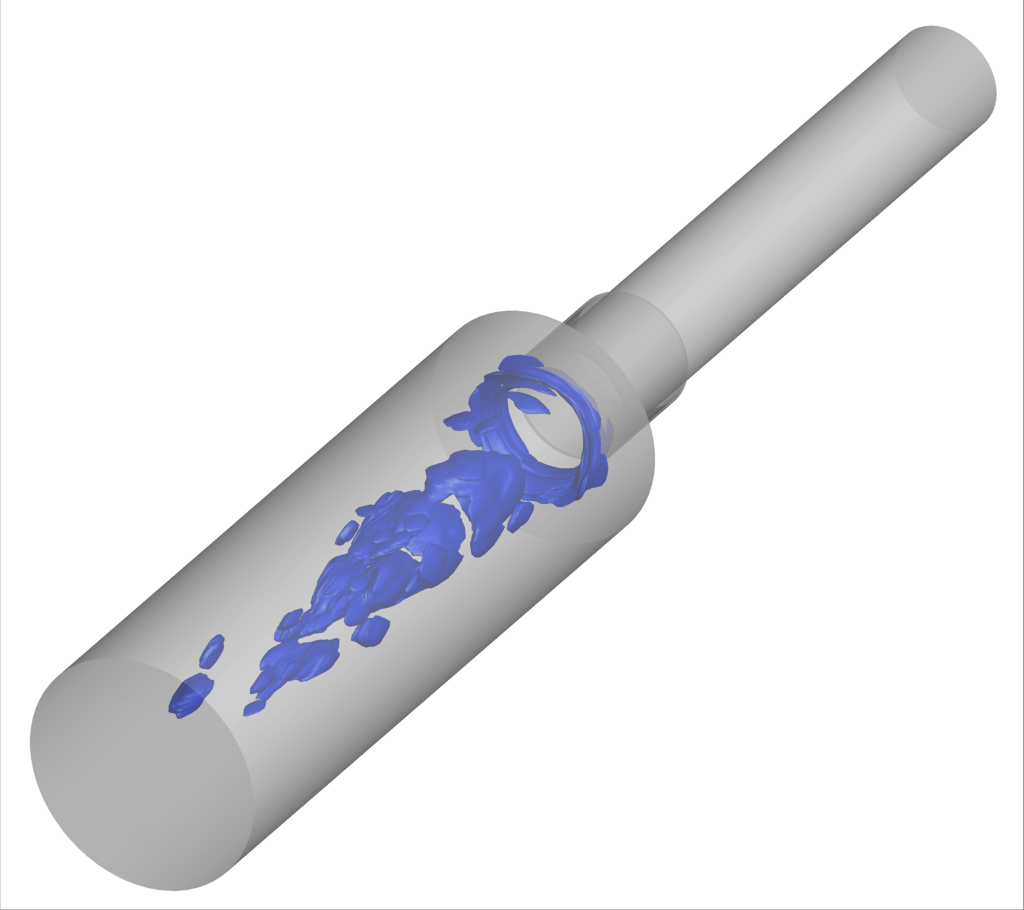
\includegraphics[width=0.99\linewidth,trim={0.5em 0.5em 0.5em 0.5em},clip]{Chapters/AdaptiveResults/Images/cvrc/iblank/iblank_iso_1075.png}
	\end{minipage}
	\begin{minipage}{0.45\linewidth}
		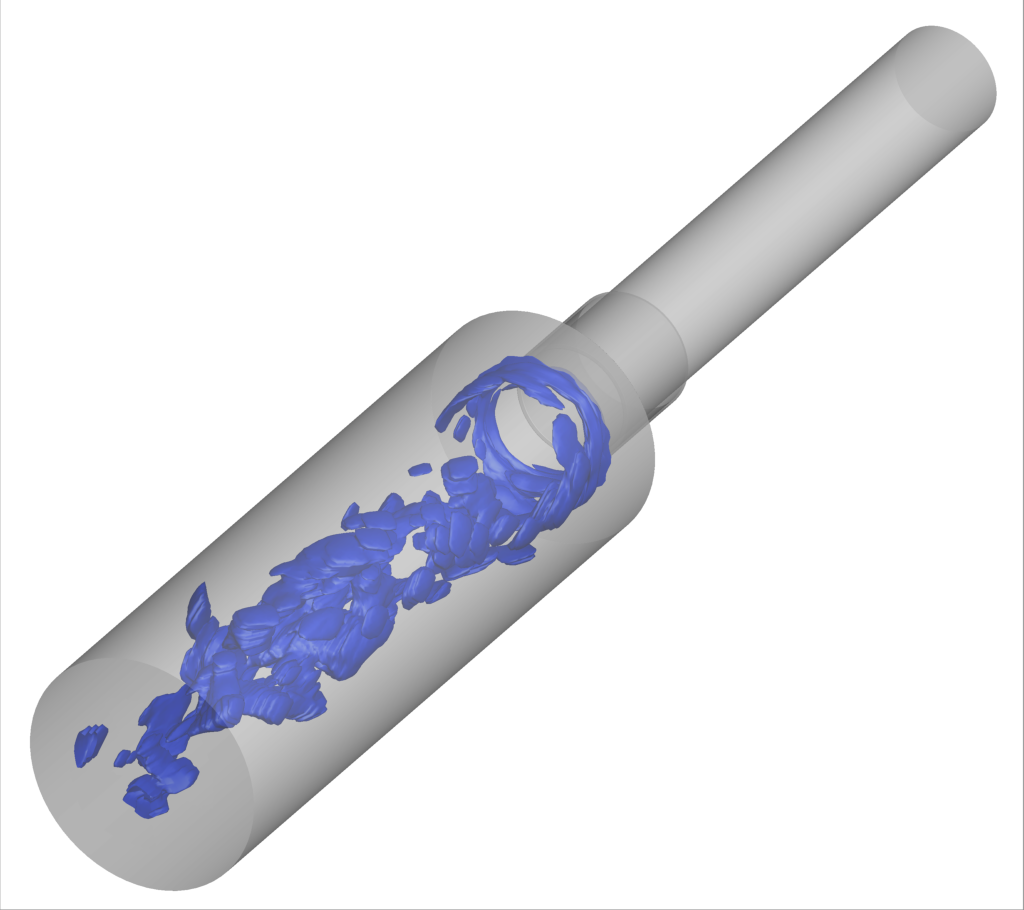
\includegraphics[width=0.99\linewidth,trim={0.5em 0.5em 0.5em 0.5em},clip]{Chapters/AdaptiveResults/Images/cvrc/iblank/iblank_iso_1100.png}
	\end{minipage}
	\caption{\label{fig:cvrcAdaptiveIBlankIso}Directly-sampled cell isosurfaces, $\numSamps = XXX\% \times \numDOF$, $\numPrimModes = 5$, XXX.}
\end{figure}

\begin{figure}
    \centering
    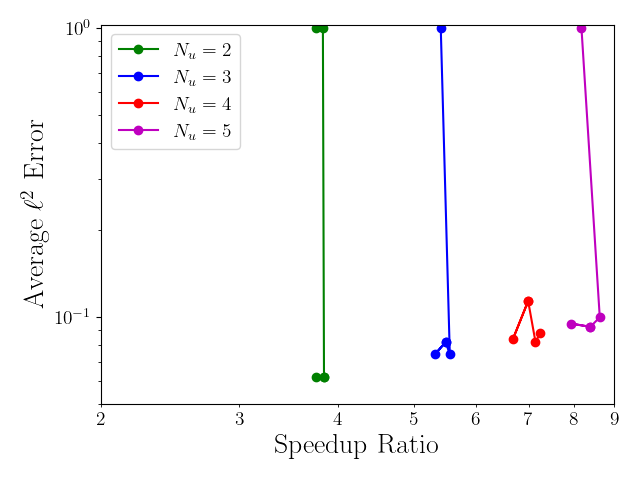
\includegraphics[width=0.5\linewidth]{Chapters/AdaptiveResults/Images/cvrc/pareto_wrt_iters_Average_errorRaw_pareto.png}
    \caption{CVRC adaptive HPROM time-average error vs. computational speedup, various $\updateFreq$.}
\end{figure}